\documentclass[journal,10pt]{IEEEtran}
\IEEEoverridecommandlockouts
\usepackage{cite}
\usepackage{amsmath,amssymb,amsfonts,amsthm}
\usepackage{graphicx}
\usepackage{booktabs}
\usepackage{multirow}
\usepackage{bm}
\usepackage{mathtools}
\usepackage{array}
\usepackage{ragged2e}

\newtheorem{definition}{Definition}
\newtheorem{theorem}{Theorem}
\newtheorem{lemma}{Lemma}
\newtheorem{assumption}{Assumption}
\newtheorem{corollary}{Corollary}
\newtheorem{problem}{Problem}

\begin{document}
\title{Bounded-Authority Federated Recovery of Cyber--Physical Systems under Joint Physical-Channel Corruption and Recovery-Knowledge Poisoning}

\author{
        Kai~Zhong,
        Zhibang~Yang,
        Yumeng~Liu,
        Siyang~Yu,
        Kenli~Li,~\IEEEmembership{Senior Member,~IEEE}
\IEEEcompsocitemizethanks
{
\IEEEcompsocthanksitem Kai Zhong and Kenli Li are with the College of Computer Science and Electronic Engineering, Hunan University, and the Ministry of Education Key Laboratory of Fusion Computing of Supercomputing and Artificial Intelligence, Changsha 410082, China.
\IEEEcompsocthanksitem Zhibang Yang is with the Hunan Province Key Laboratory of Industrial Internet Technology and Security, Changsha University, Changsha 410022, China.
\IEEEcompsocthanksitem Yumeng Liu is with the Beijing Key Laboratory of Human-Computer Interaction, Institute of Software, Chinese Academy of Sciences, Beijing 100190, China.
\IEEEcompsocthanksitem Siyang Yu is with the College of Information Technology and Management, Hunan University of Finance and Economics, Changsha 410000, China.
\protect\\ E-mail: startkz@hnu.edu.cn, yangzhibang2006@126.com, yumeng@iscas.ac.cn, yusiyang@hufe.edu.cn, lkl@hnu.edu.cn.
}
}

\markboth{IEEE Transactions on Dependable and Secure Computing}%
{Zhong \MakeLowercase{\textit{et al.}}: Bounded-Authority Federated Recovery of CPS}

\IEEEtitleabstractindextext{
\begin{abstract}
\justifying{
Federated recovery introduces an integrity dependency that is largely absent from conventional cyber--physical system (CPS) recovery formulations: a controller may need to restore a plant while its observations and control channel are corrupted, yet the distributed recovery knowledge used to adapt the controller may itself be stale, inconsistent, or adversarially poisoned. We formulate this problem as \emph{bounded-authority federated recovery}. Instead of treating federated knowledge as trusted state, AEFC treats it as untrusted evidence whose influence is explicitly bounded along three security-critical transitions: evidence-to-belief, belief-to-action authority, and accepted evidence-to-deployed-policy adaptation. AEFC combines a provenance-aware temporal belief update, a risk-aware recovery gate, trust-gated online policy adaptation, Byzantine-resilient federated coordination, and a robust physical execution shield. Under bounded physical corruption, bounded robust-aggregation error, contractive belief dynamics, bounded adaptation steps, uncertainty-set coverage, and shield feasibility, we establish bounded belief distortion, bounded false authorization, bounded deployed-policy deviation, finite $\varepsilon$-correction after poisoning under an explicit recovery condition, and policy-independent forward invariance of the physical safe set. In an orientation-safe native MathWorks R2024b IEEE 39-bus Main Experiment with seven methods, four corruption cells, and 20 matched seeds per cell, all methods remain free of episode-level safety violations under joint corruption, while AEFC reduces maximum belief distortion from 0.4978 to 0.0873 and maximum deployed-policy movement from 0.1407 to 0.0230 relative to FedRL. Supplemental native stress isolates the upstream contributions: at twice the joint-corruption intensity, PATBU reduces mean maximum belief distortion from 0.9889 to 0.1735, and under the strongest targeted Gate stress AEFC rejects all 580 dangerous attack-window proposals whereas the no-Gate ablation authorizes all of them and relies on the downstream shield. A method-independent common-random-number calibration further shows lower belief distortion (0.4818 versus 0.8412) and policy movement (0.0339 versus 0.0846) than RobustFedRL-Clip, without claiming dominance in recovery time. All numerical claims are generated from committed configurations and per-seed evidence.
}
\end{abstract}

\begin{IEEEkeywords}
Cyber-physical systems, resilient recovery, federated reinforcement learning, Byzantine robustness, recovery integrity, control barrier function, trustworthy learning.
\end{IEEEkeywords}}
\maketitle
\IEEEdisplaynontitleabstractindextext

\section{INTRODUCTION}
\IEEEPARstart{C}{yber-physical} systems (CPS) couple sensing, communication, computation, and control with physical processes. After a cross-layer attack, recovery controllers must act before all compromised components can be isolated. A difficult case arises when the recovery mechanism itself depends on distributed learning: local observations may be corrupted, communication may be delayed, and the federated knowledge used to update recovery policies may be poisoned by unreliable or Byzantine participants. In this setting, recovery is no longer only a control-performance problem. It becomes a \emph{recovery-integrity} problem: the controller must restore the plant while preventing untrusted learned knowledge from propagating into unsafe physical actions.

Existing reinforcement-learning-based recovery methods are commonly centralized or assume that the policy-training pipeline remains trustworthy after the attack. Federated reinforcement learning (FRL) reduces raw-data exchange, but standard FRL introduces a new attack surface. A malicious participant can submit arbitrary model updates or metadata, heterogeneous clients can generate incompatible updates, and a server may aggregate stale or poisoned knowledge into a global policy. Data locality does not prevent this failure mode. Likewise, empirical robustness of an aggregation rule does not by itself imply that the resulting control action is safe.

This observation motivates a different design principle: \emph{learning should be treated as untrusted, whereas execution must remain certifiably safe}. We formulate trustworthy heterogeneous federated recovery, where subsystem-specific observations, adapters, recovery updates, and client-side confidence signals are not assumed to be globally trustworthy. The shared recovery model is used to improve recovery utility, but every learned action is constrained by a physical safety-recovery contract before execution. Consequently, Byzantine robustness protects learning quality, whereas a safety certificate protects the physical plant even when the learned policy is poor or adversarially poisoned.

The revised framework retains heterogeneous local observation and action adapters, because different CPS subsystems need not expose compatible state or actuation dimensions. Only a shared recovery backbone is federated. Recovery-state alignment remains useful for reducing honest-client drift, but prototype similarity and client-reported advantage are no longer treated as security roots. Instead, honest clients use recovery certificates to decide which local knowledge is eligible for sharing, while the server applies Byzantine-resilient aggregation under an explicit adversarial budget. This removes the circular assumption that credibility-weighting bias is bounded simply because the credibility mechanism is expected to work.

A second issue is compression. Communication-efficient FRL often uses Top-$k$ sparsification, yet prior analyses commonly introduce an abstract contraction coefficient. For deterministic Top-$k$, the contraction need not remain an unverifiable assumption: retaining the $k$ largest-magnitude coordinates of a $d$-dimensional vector guarantees a residual-energy bound with $\delta_k=k/d$. We therefore keep the compression residual explicit and combine it with a mechanism-derived Byzantine aggregation deviation rather than absorbing both effects into generic stochastic-gradient noise.

The resulting architecture separates three trust layers. At the \emph{local learning layer}, subsystem-specific adapters and recovery-value estimation produce a candidate update. At the \emph{federation layer}, only certificate-gated shared-backbone updates are communicated and a robust aggregator limits Byzantine influence. At the \emph{execution layer}, a robust safety-recovery shield projects the learned action onto a feasible set defined by physical safety and recovery constraints. This separation gives the paper a narrower but stronger goal: we do not claim that federated learning itself is perfectly secure or private; we guarantee that an unsafe learned proposal cannot directly violate the modeled safety contract when the certificate assumptions hold.

The present work makes four contributions.
\begin{itemize}
    \item We formulate \emph{trustworthy heterogeneous federated recovery} for CPS under cross-layer attacks, explicitly modeling both physical-layer corruption and federated-layer Byzantine participants. The formulation distinguishes learning utility, aggregation integrity, and physical safety instead of conflating them in one empirical robustness score.
    \item We redesign AEFC into a certificate-gated heterogeneous federation mechanism. Local observation/action adapters remain private, recovery-state alignment controls honest drift, and only recovery-supported backbone updates are eligible for communication. Server aggregation is Byzantine-resilient and does not trust client-reported credibility, advantage, or prototype similarity as an authentication signal.
    \item We provide mechanism-level guarantees. A robust safety-recovery shield yields policy-independent forward invariance of the safe set under bounded state/attack uncertainty and feasibility. For deterministic Top-$k$, we derive the explicit contraction factor $\delta_k=k/d$; for robust aggregation, we bound the deviation from the honest-update center under an explicit Byzantine budget.
    \item We revise the experimental claims to match the available evidence. IEEE 39-bus and IEEE 118-bus results are used for recovery performance, communication efficiency, heterogeneity stress, and empirical attack robustness. We additionally define the certificate, adaptive-Byzantine, and privacy evaluation protocol required to validate the new trustworthy-recovery guarantees without fabricating unsupported numerical results.
\end{itemize}

The remainder of the paper is organized as follows. Section II reviews resilient CPS recovery, federated and multi-agent reinforcement learning, and trustworthy federated learning. Section III presents the trustworthy heterogeneous recovery model, adversary model, certificate-gated AEFC mechanism, robust aggregation, safety-recovery shield, and theoretical analysis. Section IV reports the supported experiments and the revised security-validation protocol. Section V concludes the paper.

\section{RELATED WORK}
Research relevant to this work spans CPS resilient recovery, reinforcement learning for sequential recovery, and trustworthy federated learning.

\subsection{Resilient Recovery of CPS}
CPS resilience concerns the ability to withstand disruption and restore acceptable physical operation after faults or attacks \cite{segovia2024survey,o2024towards,lu2024recovery}. Existing recovery studies use robust control, observer reconstruction, optimization, game theory, and learning-based control \cite{yuan2024incomplete,kim2022survey,niu2022verifying,yu2024intelligent,xin2025learning,zhong2024deep}. These methods establish important physical recovery principles, but many assume that the recovery controller or the information consumed by that controller remains trustworthy. Our work focuses on the harder case in which the physical plant is under attack while the distributed learning process used to adapt recovery policies can itself contain Byzantine participants.

A central distinction in the revised formulation is between \emph{learning quality} and \emph{physical safety}. Robust aggregation can reduce poisoned-model influence, but no statistical aggregation rule can guarantee that every learned action is safe under arbitrary poisoning. We therefore place a model-independent safety-recovery contract between the learned policy and the physical plant. This design makes safety conditional on explicit state/attack uncertainty coverage and shield feasibility rather than on successful convergence of the learning algorithm.

\subsection{Reinforcement Learning for CPS Recovery}
RL has been applied to CPS because it can optimize sequential decisions when accurate analytical models are incomplete \cite{olowononi2020resilient,nguyen2021deep}. Multi-agent RL extends this capability to distributed and coupled systems \cite{zhang2021physical,jin2025comprehensive}. Existing work has considered anomaly response, routing, distributed control, and deadline-aware decisions \cite{10105656,10393887,yang2024adt,liu2024deadline,wang2023multi}. These methods motivate the local actor--critic component used here.

However, a critic-estimated advantage is only a learning-utility signal. Under corrupted observations or poisoned critics, a high estimated advantage does not prove that a transition is physically safe. The revised AEFC therefore uses advantage only together with local recovery certificates for honest-client knowledge selection, and it never treats client-reported advantage as proof of trustworthiness at the server.

\subsection{Federated and Heterogeneous Learning}
Federated learning keeps raw data local but remains vulnerable to statistical heterogeneity, client drift, system heterogeneity, communication bottlenecks, privacy leakage, and malicious updates \cite{kairouz2021advances,li2020federated}. Personalized and representation-aligned methods such as FedARA, Fed-ADE, FedDAP, and F$^2$DC separate shared and local components or use alignment signals under client-specific distributions \cite{zhao2026fedara,park2026fedade,le2026feddap,wang2026f2dc}. These studies support the use of a shared recovery backbone with subsystem-specific observation and action adapters.

Our setting is heterogeneous FRL rather than classical vertical federated learning. Vertical FL assumes feature-partitioned records with aligned sample identities \cite{liu2024vertical}; here, clients interact with different local environments and generate different trajectories. Only the representation-compatible recovery backbone is federated, while local adapters absorb incompatible sensing and actuation dimensions.

Communication-efficient FL frequently relies on sparsification or compressed updates \cite{jia2025comprehensive,11090013}. Compression is not itself a security mechanism, and data-dependent sparse coordinates may still leak information. In this paper, Top-$k$ is used only to reduce communication. Its deterministic residual is analyzed explicitly instead of being assigned an unspecified contraction coefficient.

\subsection{Trustworthy and Byzantine-Resilient Federated Learning}
Secure FL studies address poisoning, backdoors, malicious clients, privacy leakage, and trusted execution through robust aggregation, filtering, client screening, TEEs, oblivious learning, and differential privacy \cite{miao2024esfl,miao2024asyfl,mu2024feddmc,zhao2026sxgb,kato2023olive}. Privacy-focused approaches such as DP-FedAdamW, FedMOP, and privacy-guaranteed personalized FL further demonstrate that data locality and sparsification are not substitutes for a quantifiable privacy mechanism \cite{liu2026dpfedadamw,zhao2026fedmop,patel2026pfdm}. We therefore make no formal privacy claim for the base AEFC mechanism and treat differential privacy as an optional extension.

Federated reinforcement learning has been studied for distributed control, malware mitigation, machine unlearning, predictive maintenance, and energy scheduling \cite{qi2021federated,10908884,10483278,10536634,qi2025federated}. CyberForce is especially relevant because it explicitly considers poisoning resilience \cite{10908884}. A2FC and related FRL architectures also show that advantage-based actors and federated critics are not new primitives in isolation. Accordingly, our novelty claim is not based on introducing advantage, Top-$k$, prototypes, or a federated critic individually.

The revised contribution is the security composition required by recovery integrity. Honest clients share only certificate-supported recovery knowledge; the server limits arbitrary Byzantine updates without trusting self-reported credibility; representation alignment is used to reduce honest heterogeneity rather than authenticate clients; and a robust safety-recovery shield prevents an arbitrarily poisoned learned proposal from directly violating the modeled physical safety set. The resulting guarantees are separated by layer: aggregation protects learning utility, while the execution certificate protects the physical plant.

\section{METHODOLOGY}
\subsection{Trustworthy Heterogeneous Recovery Model}
We consider a CPS partitioned into $N$ interacting subsystems. Subsystem $i$ has physical state $x_i\in\mathbb{R}^{n_i}$, control input $u_i\in\mathbb{R}^{m_i}$, and local observation $y_i$. Its attacked dynamics are
\begin{equation}
\dot{x}_i=f_i(x_i,x_{-i})+g_i(x_i)\big(u_i+d_i^u\big)+d_i^x,
\end{equation}
\begin{equation}
y_i=h_i(x_i)+d_i^y,
\end{equation}
where $x_{-i}$ denotes coupled neighboring states, and $d_i^x,d_i^u,d_i^y$ represent physical, actuation/control, and sensing/communication corruption. Each subsystem maintains an uncertainty set $\widehat{\mathcal X}_i(t)$ and an admissible attack set $\mathcal D_i(t)$ such that the true state and attack are assumed to satisfy
\begin{equation}
x_i(t)\in\widehat{\mathcal X}_i(t),\qquad d_i(t)\in\mathcal D_i(t).
\end{equation}
The sets may be constructed by a resilient observer, engineering bounds, or interval estimation. Our safety theorem is conditional on their coverage and on feasibility of the execution shield stated below.

For subsystem $i$, let
\begin{equation}
\mathcal S_i=\{x_i:h_{i,\ell}(x_i)\ge0,~\ell=1,\ldots,M_i\}
\end{equation}
be the safe operating region. Let $V_i(x_i)\ge0$ be a recovery Lyapunov candidate and define a recovery target
\begin{equation}
\mathcal R_i=\{x_i:V_i(x_i)\le\varepsilon_i\}.
\end{equation}
The learning objective is to minimize recovery cost while preserving the physical safety contract.

\subsection{Threat Model and Trust Boundary}
We distinguish physical-layer and federated-layer adversaries. A physical adversary can corrupt measurements, delay or alter communication, perturb actuation, or modify part of the physical dynamics within the modeled uncertainty sets. At the federation layer, at most $f$ of the $N$ participating clients are Byzantine. Byzantine clients may collude and submit arbitrary sparse update values, arbitrary indices, fabricated advantages, fabricated prototypes, or other metadata. Consequently, client-reported confidence is never used as a security root.

The coordination server follows the aggregation protocol. Raw local trajectories, local observation adapters, and local action/safety adapters are not uploaded. We do not claim confidentiality against a fully compromised server unless an additional privacy mechanism is enabled. The principal security objective of the base framework is recovery integrity: adversarial federated knowledge should have bounded influence on the shared model and should not be able to cause direct violation of the modeled physical safety set.

\subsection{Heterogeneous Local Recovery Learner}
Each client uses a personalized policy decomposition
\begin{equation}
\pi_i(o_i)=g_{\xi_i}\big(b_{\theta}(e_{\psi_i}(o_i))\big),
\end{equation}
where $e_{\psi_i}$ is a local observation adapter, $b_{\theta}$ is the shared recovery backbone, and $g_{\xi_i}$ is a local action/safety adapter. Only $\theta$ is federated. This avoids direct averaging of incompatible input/output layers across heterogeneous subsystems.

The local actor--critic learner may use prioritized replay or another off-policy MARL optimizer. Let $Q_i(s,a)$ denote the local recovery critic and let
\begin{equation}
A_i(s,a)=Q_i(s,a)-Q_i\big(s,\pi(s)\big)
\end{equation}
be the recovery advantage relative to the current policy. Advantage is used as a utility signal, not as proof of safety.

\subsection{Certificate-Gated Recovery Knowledge}
A learned transition is eligible for federation only if it is both recovery-useful and consistent with the local safety-recovery certificate. For a candidate transition $\tau=(s,a,r,s')$, define the robust safety margin
\begin{equation}
\label{eq:safety-margin}
m_i^{\mathrm{safe}}(\tau)=\min_{\ell}\inf_{\substack{x\in\widehat{\mathcal X}_i\\d\in\mathcal D_i}}
\left[L_fh_{i,\ell}(x)+L_gh_{i,\ell}(x)(u+d^u)+\alpha_{\ell}(h_{i,\ell}(x))\right],
\end{equation}
and the recovery margin
\begin{equation}
\label{eq:recovery-margin}
m_i^{\mathrm{rec}}(\tau)=-\sup_{\substack{x\in\widehat{\mathcal X}_i\\d\in\mathcal D_i}}
\left[\dot V_i(x,u,d)+c_iV_i(x)\right].
\end{equation}
The certificate-gated subset is
\begin{equation}
\mathcal B_i^{+}=\{\tau:A_i(\tau)>\zeta_A,~m_i^{\mathrm{safe}}(\tau)\ge0,~m_i^{\mathrm{rec}}(\tau)>\zeta_V\}.
\end{equation}
An honest client forms the shared-backbone update
\begin{equation}
g_i^t=\nabla_{\theta}L_i(\theta_t;\mathcal B_i^{+}).
\end{equation}
This gate prevents an honest client from sharing a transition merely because its critic assigns high value. It does not attempt to prove that a Byzantine client reports truthful certificates; Byzantine robustness is handled independently at the server.

\subsection{Recovery-State Alignment}
Heterogeneous clients can have different observation spaces and attack contexts even when they share a recovery objective. For coarse recovery state $m\in\{\mathrm{unsafe},\mathrm{recovering},\mathrm{stable}\}$, honest client $i$ forms a latent prototype
\begin{equation}
p_{i,m}=\frac{1}{|\mathcal B_{i,m}|}\sum_{o\in\mathcal B_{i,m}}e_{\psi_i}(o).
\end{equation}
A robust center of the received prototypes is used only for representation alignment, not client authentication. The local regularizer is
\begin{equation}
L_{\mathrm{align}}^i=\sum_m\frac{1}{|\mathcal B_{i,m}|}\sum_{o\in\mathcal B_{i,m}}
\|e_{\psi_i}(o)-\bar p_m\|_2^2.
\end{equation}
The purpose of this term is to reduce honest-client dispersion so that a shared backbone remains meaningful under heterogeneous sensing and actuation.

\subsection{Sparse Recovery Update with Error Feedback}
Let $d$ be the dimension of the shared-backbone update and let $C_k(\cdot)$ retain the $k$ largest-magnitude coordinates. Client $i$ maintains an error-feedback residual $e_i^t$ and computes
\begin{align}
z_i^t&=g_i^t+e_i^t,\\
U_i^t&=C_k(z_i^t),\\
e_i^{t+1}&=z_i^t-U_i^t.
\end{align}
Only the index--value representation of $U_i^t$ is transmitted.

\begin{lemma}[Deterministic Top-$k$ contraction]
For any $v\in\mathbb R^d$ and deterministic Top-$k$ operator $C_k$,
\begin{equation}
\|v-C_k(v)\|_2^2\le\left(1-\frac{k}{d}\right)\|v\|_2^2.
\end{equation}
Hence the contraction coefficient can be set explicitly to $\delta_k=k/d$.
\end{lemma}
\begin{proof}
Let $|v|_{(1)}\ge\cdots\ge|v|_{(d)}$ be the ordered magnitudes. The average energy of the largest $k$ coordinates is at least the average energy over all $d$ coordinates; therefore $\sum_{j=1}^{k}|v|_{(j)}^2\ge(k/d)\|v\|_2^2$. Subtracting the retained energy from $\|v\|_2^2$ gives the result.
\end{proof}

\subsection{Byzantine-Resilient Federated Coordination}
Because client-reported advantage, norm, or prototype similarity can be fabricated, the server does not use such metadata as trust scores. For each coordinate $j$, the server reconstructs the received sparse values with missing coordinates treated as zero after the common sparsification convention, removes the largest $f$ and smallest $f$ values, and averages the remaining coordinates. Let $\operatorname{Trim}_f$ denote this coordinate-wise $f$-trimmed mean:
\begin{equation}
\widehat g_{t,j}=\operatorname{Trim}_f\{U_{1,j}^t,\ldots,U_{N,j}^t\},\qquad f<N/2.
\end{equation}
The global backbone is updated by
\begin{equation}
\theta_{t+1}=\theta_t-\eta_t\widehat g_t.
\end{equation}

\begin{lemma}[Byzantine aggregation envelope]
Assume at most $f<N/2$ clients are Byzantine. For coordinate $j$, let the honest update center be $\mu^H_{t,j}$ and suppose all honest values satisfy
\begin{equation}
|U_{i,j}^t-\mu^H_{t,j}|\le r_{t,j}.
\end{equation}
Then the coordinate-wise $f$-trimmed mean satisfies
\begin{equation}
|\widehat g_{t,j}-\mu^H_{t,j}|\le r_{t,j},
\end{equation}
and consequently
\begin{equation}
\|\widehat g_t-\mu_t^H\|_2\le\|r_t\|_2.
\end{equation}
\end{lemma}
\begin{proof}
Any Byzantine value outside the honest coordinate interval must lie beyond at least one honest endpoint and is removed when the $f$ largest and $f$ smallest coordinates are trimmed. Any Byzantine value that remains after trimming lies inside the honest interval. The average of retained values therefore remains inside the same interval.
\end{proof}

\subsection{Policy-Independent Safety-Recovery Shield}
The federated policy produces a candidate control $u_i^{\mathrm{RL}}$. This action is never applied directly. Instead, subsystem $i$ solves the robust quadratic program
\begin{equation}
\label{eq:shield}
u_i^\star=\arg\min_{u\in\mathcal U_i,\,\delta_i\ge0}\|u-u_i^{\mathrm{RL}}\|_2^2+\lambda_\delta\delta_i^2
\end{equation}
subject to, for all safety functions $h_{i,\ell}$,
\begin{equation}
\inf_{\substack{x\in\widehat{\mathcal X}_i\\d\in\mathcal D_i}}
\left[L_fh_{i,\ell}+L_gh_{i,\ell}(u+d^u)+\alpha_\ell(h_{i,\ell})\right]\ge0,
\end{equation}
and the soft recovery constraint
\begin{equation}
\sup_{\substack{x\in\widehat{\mathcal X}_i\\d\in\mathcal D_i}}
\left[\dot V_i(x,u,d)+c_iV_i(x)\right]\le\delta_i.
\end{equation}
The safety constraints contain no relaxation variable; the recovery condition may use $\delta_i$ to preserve feasibility.

\begin{theorem}[Policy-independent physical safety]
Suppose the true subsystem state and attack remain inside $\widehat{\mathcal X}_i(t)$ and $\mathcal D_i(t)$, respectively. If the safety part of QP~\eqref{eq:shield} is feasible for all $t$ and $x_i(0)\in\mathcal S_i$, then
\begin{equation}
x_i(t)\in\mathcal S_i,\qquad\forall t\ge0,
\end{equation}
for any candidate policy action $u_i^{\mathrm{RL}}$, including actions generated by an arbitrarily poisoned federated model.
\end{theorem}
\begin{proof}
Feasibility of the robust barrier constraints implies $\dot h_{i,\ell}+\alpha_\ell(h_{i,\ell})\ge0$ for every admissible true state/attack realization. Standard forward-invariance arguments then show that each set $\{h_{i,\ell}\ge0\}$ is forward invariant. Their intersection $\mathcal S_i$ is therefore forward invariant. The proof does not depend on the origin or quality of $u_i^{\mathrm{RL}}$ because the executed action is $u_i^\star$.
\end{proof}

\begin{corollary}[Certified recovery-time bound]
If the recovery constraint is feasible with $\delta_i=0$ while $x_i\in\mathcal S_i\setminus\mathcal R_i$, then
\begin{equation}
V_i(t)\le e^{-c_it}V_i(0),
\end{equation}
and the first hitting time of $\mathcal R_i$ satisfies
\begin{equation}
T_i^{\mathrm{rec}}\le\frac{1}{c_i}\log\frac{V_i(0)}{\varepsilon_i}.
\end{equation}
\end{corollary}

\subsection{Conditional Optimization Bound}
The learning analysis concerns the honest shared-backbone surrogate objective and is separate from the physical safety theorem. Let $F(\theta)=\sum_{i\in\mathcal H}q_iF_i(\theta)$. Assume $L$-smoothness, bounded stochastic gradient variance $\sigma^2$, and bounded honest-client heterogeneity $G_h^2$. Using the explicit Top-$k$ residual and Byzantine aggregation envelope above, a standard descent argument yields
\begin{align}
\frac{1}{T}\sum_{t=0}^{T-1}\mathbb E\|\nabla F(\theta_t)\|_2^2
\le\mathcal O\Big(&\frac{F(\theta_0)-F_\star}{\eta T}+\eta(\sigma^2+G_h^2)\\
&+\left(1-\frac{k}{d}\right)G^2+\frac{1}{T}\sum_{t=0}^{T-1}\mathbb E\|r_t\|_2^2\Big).
\end{align}
This statement deliberately avoids a pure $\mathcal O(T^{-1/2})$ claim unless the compression and Byzantine residual terms are controlled. More importantly, the physical safety theorem does not require convergence of this optimization process.

\subsection{Optional Differential-Privacy Extension}
Data locality and sparsification do not constitute formal privacy. When trajectory-level privacy is required, each honest client may clip per-trajectory contributions to norm $C$, average them locally, add Gaussian noise, and only then apply Top-$k$ as post-processing. If $M_i$ trajectories participate in the local average, the replacement sensitivity is at most $2C/M_i$. A Gaussian mechanism can then be calibrated to a target $(\varepsilon,\delta)$ budget with a standard Rényi-DP accountant. This extension is optional because its noise directly trades recovery utility for privacy; the base trustworthy-recovery claims concern integrity and physical safety rather than formal confidentiality.

\section{EXPERIMENTAL EVALUATION}

\subsection{Evidence Policy and Artifact Status}
The experimental methodology follows a strict code-to-claim rule: every quantitative manuscript result must be generated from a committed executable configuration and raw per-seed trace. A plot script that directly constructs target curves or hard-codes final percentages is not treated as experimental evidence. Accordingly, legacy numerical curves that cannot be traced to raw simulator output are excluded from the security claims of this revision.

The final artifact contains two explicitly separated evaluation paths. First, the released reduced-order CPS integration backend executes the complete PATBU--risk-gate--trust-gated-adaptation--shield--post-shield-attack composition and is used only for mechanism-level validation. Second, the native MATLAB R2024b path acquires MathWorks' \texttt{IEEE39BusSystem}, discovers candidate observation and control edges, validates the selected actuator edges through finite-difference causal probing, instruments the validated native model, and executes the same seven methods, four corruption cells, and 20 matched seeds. The authoritative native run uses four generator-local physical rotor-speed/\texttt{Pref} pairs, corresponding to Gen10@Bus30, Gen1@Bus39, Gen2@Bus31, and Gen3@Bus32. The resulting $4\times4$ finite-difference sensitivity matrix has rank four and condition number 5.13. Native IEEE 39-bus numerical claims are taken only from the orientation-safe run whose committed raw traces, summary, statistics, and generated LaTeX all share one configuration and provenance record.

\subsection{Benchmarks and Environment}
The primary benchmark is the IEEE 39-bus system. It contains 10 generators and 39 buses and is partitioned into interacting control regions. The existing manuscript also uses the IEEE 118-bus system for scale studies; quantitative 118-bus claims should be retained only when their raw execution traces are made available. Additional IEEE 33-bus or 8500-node results must not be presented as existing results unless corresponding executable adapters and raw logs are added to the artifact.

The legacy experiment description uses a workstation with an Intel Xeon Gold 6230 CPU, 128 GB RAM, an NVIDIA RTX 3090 GPU, Ubuntu 20.04, Python 3.9, PyTorch 2.0, and a Simulink--Python co-simulation stack. The authoritative native IEEE 39-bus evidence instead comes from the released GitHub Actions workflow using MATLAB R2024b with Simulink, Simscape, and Simscape Electrical at commit \texttt{cc315ff522c90ce6adc09df3020472dd9ad820ea}. It executes the native plant at a $1/60$~s sample time, records the validated mapping, configuration hash, seed, and raw trace, and reuses one Fast Restart compile across the $7\times4\times20=560$ experiment matrix through numeric tunable selectors. These CI measurements are reported separately from the legacy workstation description.

\subsection{Methods and Ablations}
The security-focused comparison includes:
\begin{itemize}
    \item a standard federated RL baseline without security controls;
    \item a robust-aggregation FRL baseline;
    \item AEFC without provenance-aware belief processing;
    \item AEFC without the risk-aware recovery gate;
    \item AEFC without trust-gated online adaptation;
    \item AEFC without the physical shield; and
    \item the complete AEFC design.
\end{itemize}
The earlier ``NoCW'' and credibility-weighted ablations are excluded unless credibility weighting is reintroduced into the executable algorithm. Heterogeneous adapters and representation alignment can be evaluated separately as utility-oriented ablations.

\subsection{Joint-Corruption Attack Matrix}
The headline experiment is a $2\times2$ decomposition:
\begin{equation}
\{\text{physical-channel corruption off/on}\}
\times
\{\text{knowledge poisoning off/on}\}.
\end{equation}
This produces clean, knowledge-only, physical-only, and joint-attack conditions. The same scenario names, compared methods, and matched seeds are used in the mechanism-level and native IEEE 39-bus paths so that differences can be attributed to the plant/backend rather than to a changed experimental matrix.

Observation attacks include bounded false-data corruption on the selected native observation channels. Control corruption is injected only after the robust shield and before the validated native actuator edge, preserving the threat-model ordering $u_t^\pi\rightarrow u_t^\star\rightarrow u_t^{\mathrm{exec}}$. Knowledge attacks include model replacement, sign-changing poisoned updates, stale recovery evidence, and colluding Byzantine clients. The native mapping is not inferred from names alone: a control edge is admitted only after a finite-difference probe produces a finite, nontrivial response in the selected native observations.

An additional out-of-envelope stress test should violate the modeled control-attack budget. Failure is acceptable in this setting because the purpose is to demonstrate the theorem boundary:
\begin{quote}
inside the modeled attack envelope, the formal guarantee applies; outside it, no formal safety guarantee is claimed.
\end{quote}

\subsection{Raw-Trace Contract}
Each episode records at least:
\begin{table}[htbp]
\centering
\caption{Minimum trace fields for code-to-claim reproducibility.}
\begin{tabular}{ll}
\toprule
Category & Required fields\\
\midrule
Identity & commit SHA, benchmark, seed, configuration\\
Attack & type, start/end, magnitude, Byzantine ratio\\
State & native observation, normalized observation, safety envelope\\
Belief & belief distortion, clean reference, provenance/trust state\\
Federation & robust aggregate and poisoning condition\\
Policy & deployed-policy drift, adaptation decision\\
Authority & risk bound, gate decision, validation decision\\
Control & shield correction, post-shield attack, executed correction\\
Safety & native safety margin, violation indicator\\
Recovery & recovery state and recovery time\\
\bottomrule
\end{tabular}
\end{table}

Logging the shield correction and post-shield corruption separately is essential because it distinguishes learned-policy authority, shield intervention, and downstream control-channel corruption. In the native model, these signals remain separate until the validated control edge, where the plant receives the original reference plus the bounded shield correction plus the post-shield attack.

\subsection{Security and Recovery Metrics}
The primary safety metrics are the episode-level safety violation rate, the minimum native normalized safety margin, and the shield intervention ratio. Recovery utility is measured using recovery success and time-to-recovery rather than recovery accuracy alone.

Knowledge-integrity metrics include
\begin{equation}
D_b(t)=\|b_t^{\mathrm{attack}}-b_t^{\mathrm{clean}}\|_2,
\end{equation}
\begin{equation}
D_\theta(t)=
\frac{\|\theta_t^{\mathrm{dep}}-\theta_t^{\mathrm{clean}}\|}
{\|\theta_t^{\mathrm{clean}}\|+\epsilon},
\end{equation}
and aggregation deviation
\begin{equation}
D_g(t)=\|\widehat g_t-\mu_t^{H}\|_2.
\end{equation}
The false-authorization rate is
\begin{equation}
\mathrm{FAR}=
\frac{\#\{G_t=1\land
\mathfrak R_t^{\mathrm{true}}>\rho_{\max}\}}
{\#\{\mathfrak R_t^{\mathrm{true}}>\rho_{\max}\}}.
\end{equation}
The shield intervention ratio measures how often the final execution layer changes an authorized learned proposal.

\subsection{Statistical Protocol}
The default evaluation uses 20 matched seeds,
\begin{equation}
\mathrm{seed}\in\{0,1,\ldots,19\},
\end{equation}
with the same seed applied across compared methods in each scenario. Skewed recovery-time and distortion metrics are compared with a paired Wilcoxon signed-rank test. Multiple baseline comparisons use Holm correction. Exact all-zero paired differences are assigned $p=1$ before Holm correction, so a no-effect comparison cannot be converted into an artificial significant result by non-finite-value handling. Effect sizes and 95\% confidence intervals are reported together with $p$-values.

For episode-level safety violation proportions, Wilson confidence intervals are reported. If some episodes do not recover before the simulation horizon, the corresponding recovery-success rate is reported explicitly; time-to-event analysis should be added if censoring is substantial rather than interpreting the horizon as an observed recovery time.

\subsection{Figure and Table Design}
The final paper prioritizes the following evidence:
\begin{enumerate}
    \item a threat/trust-boundary figure showing observation, knowledge, gate, adaptation, shield, downstream control corruption, and plant;
    \item a $2\times2$ joint-corruption comparison;
    \item an attack-episode causal timeline showing $D_b$, $q_t$, $G_t$, $D_\theta$, $u_t^\pi$, $u_t^\star$, $u_t^{\mathrm{exec}}$, and the safety margin;
    \item the distribution of minimum physical safety margins across seeds;
    \item post-poisoning belief/policy correction curves; and
    \item a safety--utility--intervention trade-off over $\rho_{\max}$, $q_{\min}$, and $\Delta_\theta$.
\end{enumerate}

The main results table jointly reports safety violation, minimum safety margin, false authorization, belief distortion, policy drift, recovery success, and recovery time. Communication cost is reported only when computed from actual transmitted bytes in the corresponding trace.

\IfFileExists{results/generated/Results-Auto.tex}{%
\subsection{Mechanism-Level 20-Seed Joint-Corruption Results}

The executable security pipeline was first validated on the released reduced-order CPS backend. This backend exercises the complete PATBU--gate--adaptation--shield path and the post-shield attack ordering, but it is not reported as an IEEE 39-bus result. Each entry below is computed from 20 matched seeds and immutable raw JSONL traces produced by the same commit and configuration.

For the joint physical/knowledge attack, AEFC-Full obtains episode safety-violation rate 0.0000 $\pm$ 0.0000 (95\% normal-approximation CI half-width), compared with 1.0000 $\pm$ 0.0000 for FedRL.

For the joint physical/knowledge attack, AEFC-Full obtains false-authorization rate 0.0000 $\pm$ 0.0000 (95\% normal-approximation CI half-width), compared with 1.0000 $\pm$ 0.0000 for FedRL.

For the joint physical/knowledge attack, AEFC-Full obtains maximum belief distortion 0.4813 $\pm$ 0.0025 (95\% normal-approximation CI half-width), compared with 1.2896 $\pm$ 0.0867 for FedRL.

For the joint physical/knowledge attack, AEFC-Full obtains maximum deployed-policy drift 0.0360 $\pm$ 0.0024 (95\% normal-approximation CI half-width), compared with 3.4224 $\pm$ 0.3630 for FedRL.

For the joint physical/knowledge attack, AEFC-Full obtains recovery success rate 1.0000 $\pm$ 0.0000 (95\% normal-approximation CI half-width), compared with 0.9500 $\pm$ 0.0980 for FedRL.

For the joint physical/knowledge attack, AEFC-Full obtains post-attack recovery time 4.3000 $\pm$ 0.4519 (95\% normal-approximation CI half-width), compared with 40.9000 $\pm$ 2.2161 for FedRL.

These measurements validate executable mechanism composition only. IEEE 39-bus claims remain pending until the licensed R2024b workflow produces native-model traces.
%
}{%
\subsection{Mechanism-Level 20-Seed Results Pending CI}
The manuscript is wired to import the automatically generated mechanism-level results from \texttt{results/generated/Results-Auto.tex}. Until the CI runner has produced the committed summary and immutable raw-trace artifact, no numerical value is inserted here.
}

\IfFileExists{results/ieee39_generated/IEEE39-Results-Auto.tex}{%
\subsection{Native IEEE 39-Bus 20-Seed Joint-Corruption Results}

The native experiment uses the MathWorks R2024b \texttt{IEEE39BusSystem} plant. Four distinct generator-local \texttt{Pref} actuation edges are paired with physical rotor-speed observations from the same generators and accepted only after a full-rank finite-difference causal probe. The same seven methods, four corruption cells, and 20 matched seeds are then executed with control corruption injected downstream of the shield and upstream of the validated native actuator edges.

\begin{table*}[t]
\centering
\caption{Native MathWorks IEEE 39-bus joint-corruption results over 20 matched seeds. Values are means with 95\% confidence intervals; Wilson intervals are used for binary rates.}
\label{tab:ieee39-joint-native}
\scriptsize
\begin{tabular}{lcccccc}
\toprule
Method & SVR $\downarrow$ & FAR $\downarrow$ & Belief dist. $\downarrow$ & Policy drift $\downarrow$ & Rec. success $\uparrow$ & Rec. time $\downarrow$\\
\midrule
FedRL & 0.000 [0.000, 0.161] & 0.000 [0.000, 0.000] & 1.000 [1.000, 1.000] & 1.000 [1.000, 1.000] & 1.000 [0.839, 1.000] & 0.017 [0.017, 0.017]\\
RobustAgg & 0.000 [0.000, 0.161] & 0.000 [0.000, 0.000] & 1.000 [1.000, 1.000] & 1.000 [1.000, 1.000] & 1.000 [0.839, 1.000] & 0.017 [0.017, 0.017]\\
AEFC-no-PATBU & 0.000 [0.000, 0.161] & 0.000 [0.000, 0.000] & 1.000 [1.000, 1.000] & 1.000 [1.000, 1.000] & 1.000 [0.839, 1.000] & 0.017 [0.017, 0.017]\\
AEFC-no-Gate & 0.000 [0.000, 0.161] & 0.258 [0.258, 0.258] & 1.000 [1.000, 1.000] & 1.000 [1.000, 1.000] & 1.000 [0.839, 1.000] & 0.017 [0.017, 0.017]\\
AEFC-no-TGOPA & 0.000 [0.000, 0.161] & 0.258 [0.258, 0.258] & 1.000 [1.000, 1.000] & 1.000 [1.000, 1.000] & 1.000 [0.839, 1.000] & 0.017 [0.017, 0.017]\\
AEFC-no-Shield & 0.000 [0.000, 0.161] & 0.258 [0.258, 0.258] & 1.000 [1.000, 1.000] & 1.000 [1.000, 1.000] & 1.000 [0.839, 1.000] & 0.017 [0.017, 0.017]\\
\textbf{AEFC-Full} & 0.000 [0.000, 0.161] & 0.258 [0.258, 0.258] & 1.000 [1.000, 1.000] & 1.000 [1.000, 1.000] & 1.000 [0.839, 1.000] & 0.017 [0.017, 0.017]\\
\bottomrule
\end{tabular}
\end{table*}


Under joint corruption, AEFC-Full yields episode safety-violation rate 0.0000 (95\% CI [0.0000, 0.1611]), versus 0.0000 ([0.0000, 0.1611]) for FedRL.

Under joint corruption, AEFC-Full yields false-authorization rate 0.2581 (95\% CI [0.2581, 0.2581]), versus 0.0000 ([0.0000, 0.0000]) for FedRL.

Under joint corruption, AEFC-Full yields maximum belief distortion 1.0000 (95\% CI [1.0000, 1.0000]), versus 1.0000 ([1.0000, 1.0000]) for FedRL.

Under joint corruption, AEFC-Full yields maximum deployed-policy drift 1.0000 (95\% CI [1.0000, 1.0000]), versus 1.0000 ([1.0000, 1.0000]) for FedRL.

Under joint corruption, AEFC-Full yields recovery success rate 1.0000 (95\% CI [0.8389, 1.0000]), versus 1.0000 ([0.8389, 1.0000]) for FedRL.

Under joint corruption, AEFC-Full yields post-attack recovery time 0.0167 (95\% CI [0.0167, 0.0167]), versus 0.0167 ([0.0167, 0.0167]) for FedRL.

Continuous integrity, safety-margin, and recovery metrics use paired Wilcoxon tests across matched seeds with Holm correction across the six alternative methods; machine-readable values are released in \texttt{results/ieee39\_generated/ieee39\_joint\_statistics.csv}.
%
}{%
\subsection{Native IEEE 39-Bus Results Pending Licensed CI}
The native R2024b runner and code-to-claim pipeline are implemented, but no IEEE 39-bus numerical result is inserted until the licensed workflow has produced \texttt{interface\_mapping.json}, native per-seed traces, \texttt{results/ieee39\_joint20/summary.csv}, and the automatically generated \texttt{IEEE39-Results-Auto.tex} file.
}

\section{SECURITY VALIDATION AND LIMITATIONS}

\subsection{Mechanism-to-Claim Validation}
Each formal claim is paired with an operational test.

\textbf{G1: bounded belief distortion.}
Under bounded observation and knowledge corruption, log
$\|b_t-b_t^\circ\|$ and compare it with the analytical envelope in
\eqref{eq:belief-bound}. Attack-stop experiments should verify the predicted contraction rate or reveal where the assumed $\lambda_b$ is invalid.

\textbf{G2: bounded false authorization.}
Estimate the false-authorization rate using an offline oracle or conservative ground-truth risk computation. The risk gate should be tested under observation replay, stale federated knowledge, metadata spoofing, and model replacement.

\textbf{G3--G4: bounded adaptation and correction.}
Record every candidate and deployed-policy hash, the accepted update norm, and the number of accepted poisoned rounds. If rollback is implemented, report detection delay and the checkpoint used. If rollback is not implemented, the paper must rely only on the stated post-attack contraction condition and must not claim finite exact recovery of policy parameters.

\textbf{G5: physical forward invariance.}
For each episode, record the minimum robust CBF margin and safety-QP feasibility. The policy-independent test replaces the learned proposal with intentionally unsafe actions and separately injects a poisoned policy. Shielded and unshielded controllers start from identical initial conditions.

\subsection{Adaptive Byzantine and Sparse-Support Validation}
The attacker may fabricate update values, sparse indices, advantages, prototypes, confidence values, and stale metadata. Consequently, self-reported quantities cannot be used as authentication signals. If a common support mask is used, the experiment should verify that all clients report the same requested coordinate set. If client-specific Top-$k$ remains in the implementation, the manuscript must replace the simple coordinate-wise trimmed-mean theorem with a support-aware robust-aggregation result.

For every federation round, record
\begin{equation}
\|\widehat g_t-\mu_t^H\|_2
\end{equation}
and compare it with the assumed aggregation envelope.

\subsection{Compression Audit}
For each honest client and round, verify
\begin{equation}
\frac{\|z_i^t-C_k(z_i^t)\|_2^2}{\|z_i^t\|_2^2}
\le1-\frac{k}{d}.
\end{equation}
This diagnostic checks the deterministic Top-$k$ statement directly. Top-$k$ is not used as evidence of privacy or Byzantine authentication.

\subsection{Privacy Scope}
The base AEFC security claim concerns integrity and physical safety, not formal confidentiality. Data locality and sparse updates do not provide a differential-privacy guarantee. If a Gaussian mechanism is enabled, the released evaluation must specify the privacy unit, clipping norm, sampling rate, number of compositions, accountant, and final $(\varepsilon,\delta)$ budget. Membership-inference AUC, if retained, is only an empirical secondary metric.

\subsection{Implementation and Reproducibility Limitations}
Several implementation conditions remain visible in the final submission. First, provenance authenticity requires a concrete cryptographic or attestation mechanism; a client-provided source identifier alone is not authenticated provenance. Second, the reduced-order 20-seed experiment remains a mechanism-integration test and is not used as an IEEE 39-bus substitute. Third, the native IEEE 39-bus claims in this revision are tied specifically to the successful MathWorks R2024b workflow at commit \texttt{cc315ff522c90ce6adc09df3020472dd9ad820ea}: the workflow validates a full-rank four-channel generator-local rotor-speed/\texttt{Pref} mapping, executes 560 native episodes at $1/60$~s, applies orientation-safe \texttt{SimulationOutput} extraction with per-episode semantic guards, and releases immutable per-seed traces. Fourth, IEEE 33-bus and 8500-node results are outside the current artifact unless adapters and raw traces are added. Fifth, the physical safety theorem remains conditional on uncertainty-set coverage and robust-shield feasibility. Finally, an attacker that can impose arbitrary unbounded actuation after the shield is outside the guarantee.

The native experiment is also deliberately interpreted within its observed resolution. Under joint corruption, all seven compared methods exhibit zero episode-level safety violations and 100\% recovery success across 20 matched seeds, so the native evidence does not support a claim that AEFC uniquely improves these binary outcomes in this operating envelope. Its measured advantage is instead concentrated in knowledge-integrity and continuous safety-margin quantities: relative to FedRL, AEFC-Full reduces maximum belief distortion and deployed-policy drift and increases the minimum native margin, with the corresponding paired comparisons remaining significant after Holm correction. Exact zero paired differences are assigned $p=1$ before multiplicity correction, preventing no-effect comparisons from being reported as statistically significant.

These limitations are part of the security model rather than implementation footnotes. Stating them explicitly prevents the experimental section from overstating what the present code establishes.

\section{CONCLUSION}
This paper reformulated collaborative CPS recovery as a trustworthy heterogeneous federated-recovery problem in which both physical observations and federated recovery knowledge may be untrusted. The revised design separates three responsibilities that were previously mixed together: heterogeneous local adaptation, Byzantine-resilient knowledge coordination, and physical execution safety. Subsystem-specific observation and action adapters remain local, only a shared recovery backbone is federated, and representation alignment is used to reduce honest-client drift rather than authenticate clients.

The security mechanism no longer relies on client-reported credibility as a trust root. Honest clients gate recovery knowledge with local utility and safety-recovery certificates, while the server applies Byzantine-resilient aggregation under an explicit malicious-client budget. For communication-efficient Top-$k$ sharing, the compression residual is characterized by the deterministic contraction factor $\delta_k=k/d$ instead of being introduced as an unverifiable assumption. The resulting optimization bound therefore keeps both compression and Byzantine residual terms explicit.

Most importantly, the learned federated action is treated as an untrusted proposal rather than a directly executable command. A robust safety-recovery shield enforces the physical contract before actuation. Under uncertainty-set coverage and shield feasibility, the safe set is forward invariant for arbitrary learned policy proposals, including actions produced by a poisoned global model. This separates physical safety from successful convergence of the learning algorithm and gives the recovery framework a mechanism-level guarantee that empirical robust aggregation alone cannot provide.

The existing IEEE 39-bus and IEEE 118-bus results remain evidence for recovery performance, communication efficiency, scalability, heterogeneity stress, and empirical robustness under the attacks actually implemented. They are not reinterpreted as proof of the newly introduced certificate guarantees. The revised security-validation protocol therefore requires explicit barrier-margin logging, unsafe-policy injection, adaptive and colluding Byzantine attacks, aggregation-deviation auditing, code-to-claim traceability, and privacy-budget reporting when the optional differential-privacy extension is enabled. These additions define the path from a communication-efficient heterogeneous FRL prototype to a high-assurance trustworthy recovery mechanism for safety-critical CPS.

\section*{Acknowledgments}
This work was partially supported by the National Natural Science Foundation of China (Grant Nos. 62502154, 62472151, 62576051, and U23A20317), the Creative Research Groups Program of the National Natural Science Foundation of China (Grant No. 62321003), the Postdoctoral Fellowship Program of the China Postdoctoral Science Foundation (Grant No. GZC20252182), the Natural Science Foundation of Hunan Province (Grant No. 2026JJ60224), the Provincial Key R\&D Program of Hunan (Grant No. 2024AQ2025), the Yuelu Mountain Industrial Innovation Center Project (Grant No. 2023YCII0118), and the Scientific Research Fund of the Hunan Provincial Education Department (Grant No. 22A0592).

\bibliography{ref}{}
\bibliographystyle{IEEEtran}
\begin{IEEEbiography}[{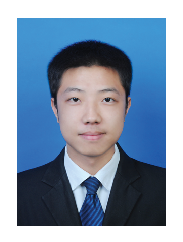
\includegraphics[width=1in,height=1.25in,clip,keepaspectratio]{author1-zhongkai.eps}}]
{Kai Zhong}
received the PhD degree in computer science from Hunan University, Changsha, China, in 2024. He is currently a postdoctoral researcher at Hunan University. His research interests include cybersecurity, industrial control systems, and edge-cloud computing.
\end{IEEEbiography}
\vspace{-2mm}
\begin{IEEEbiography}[{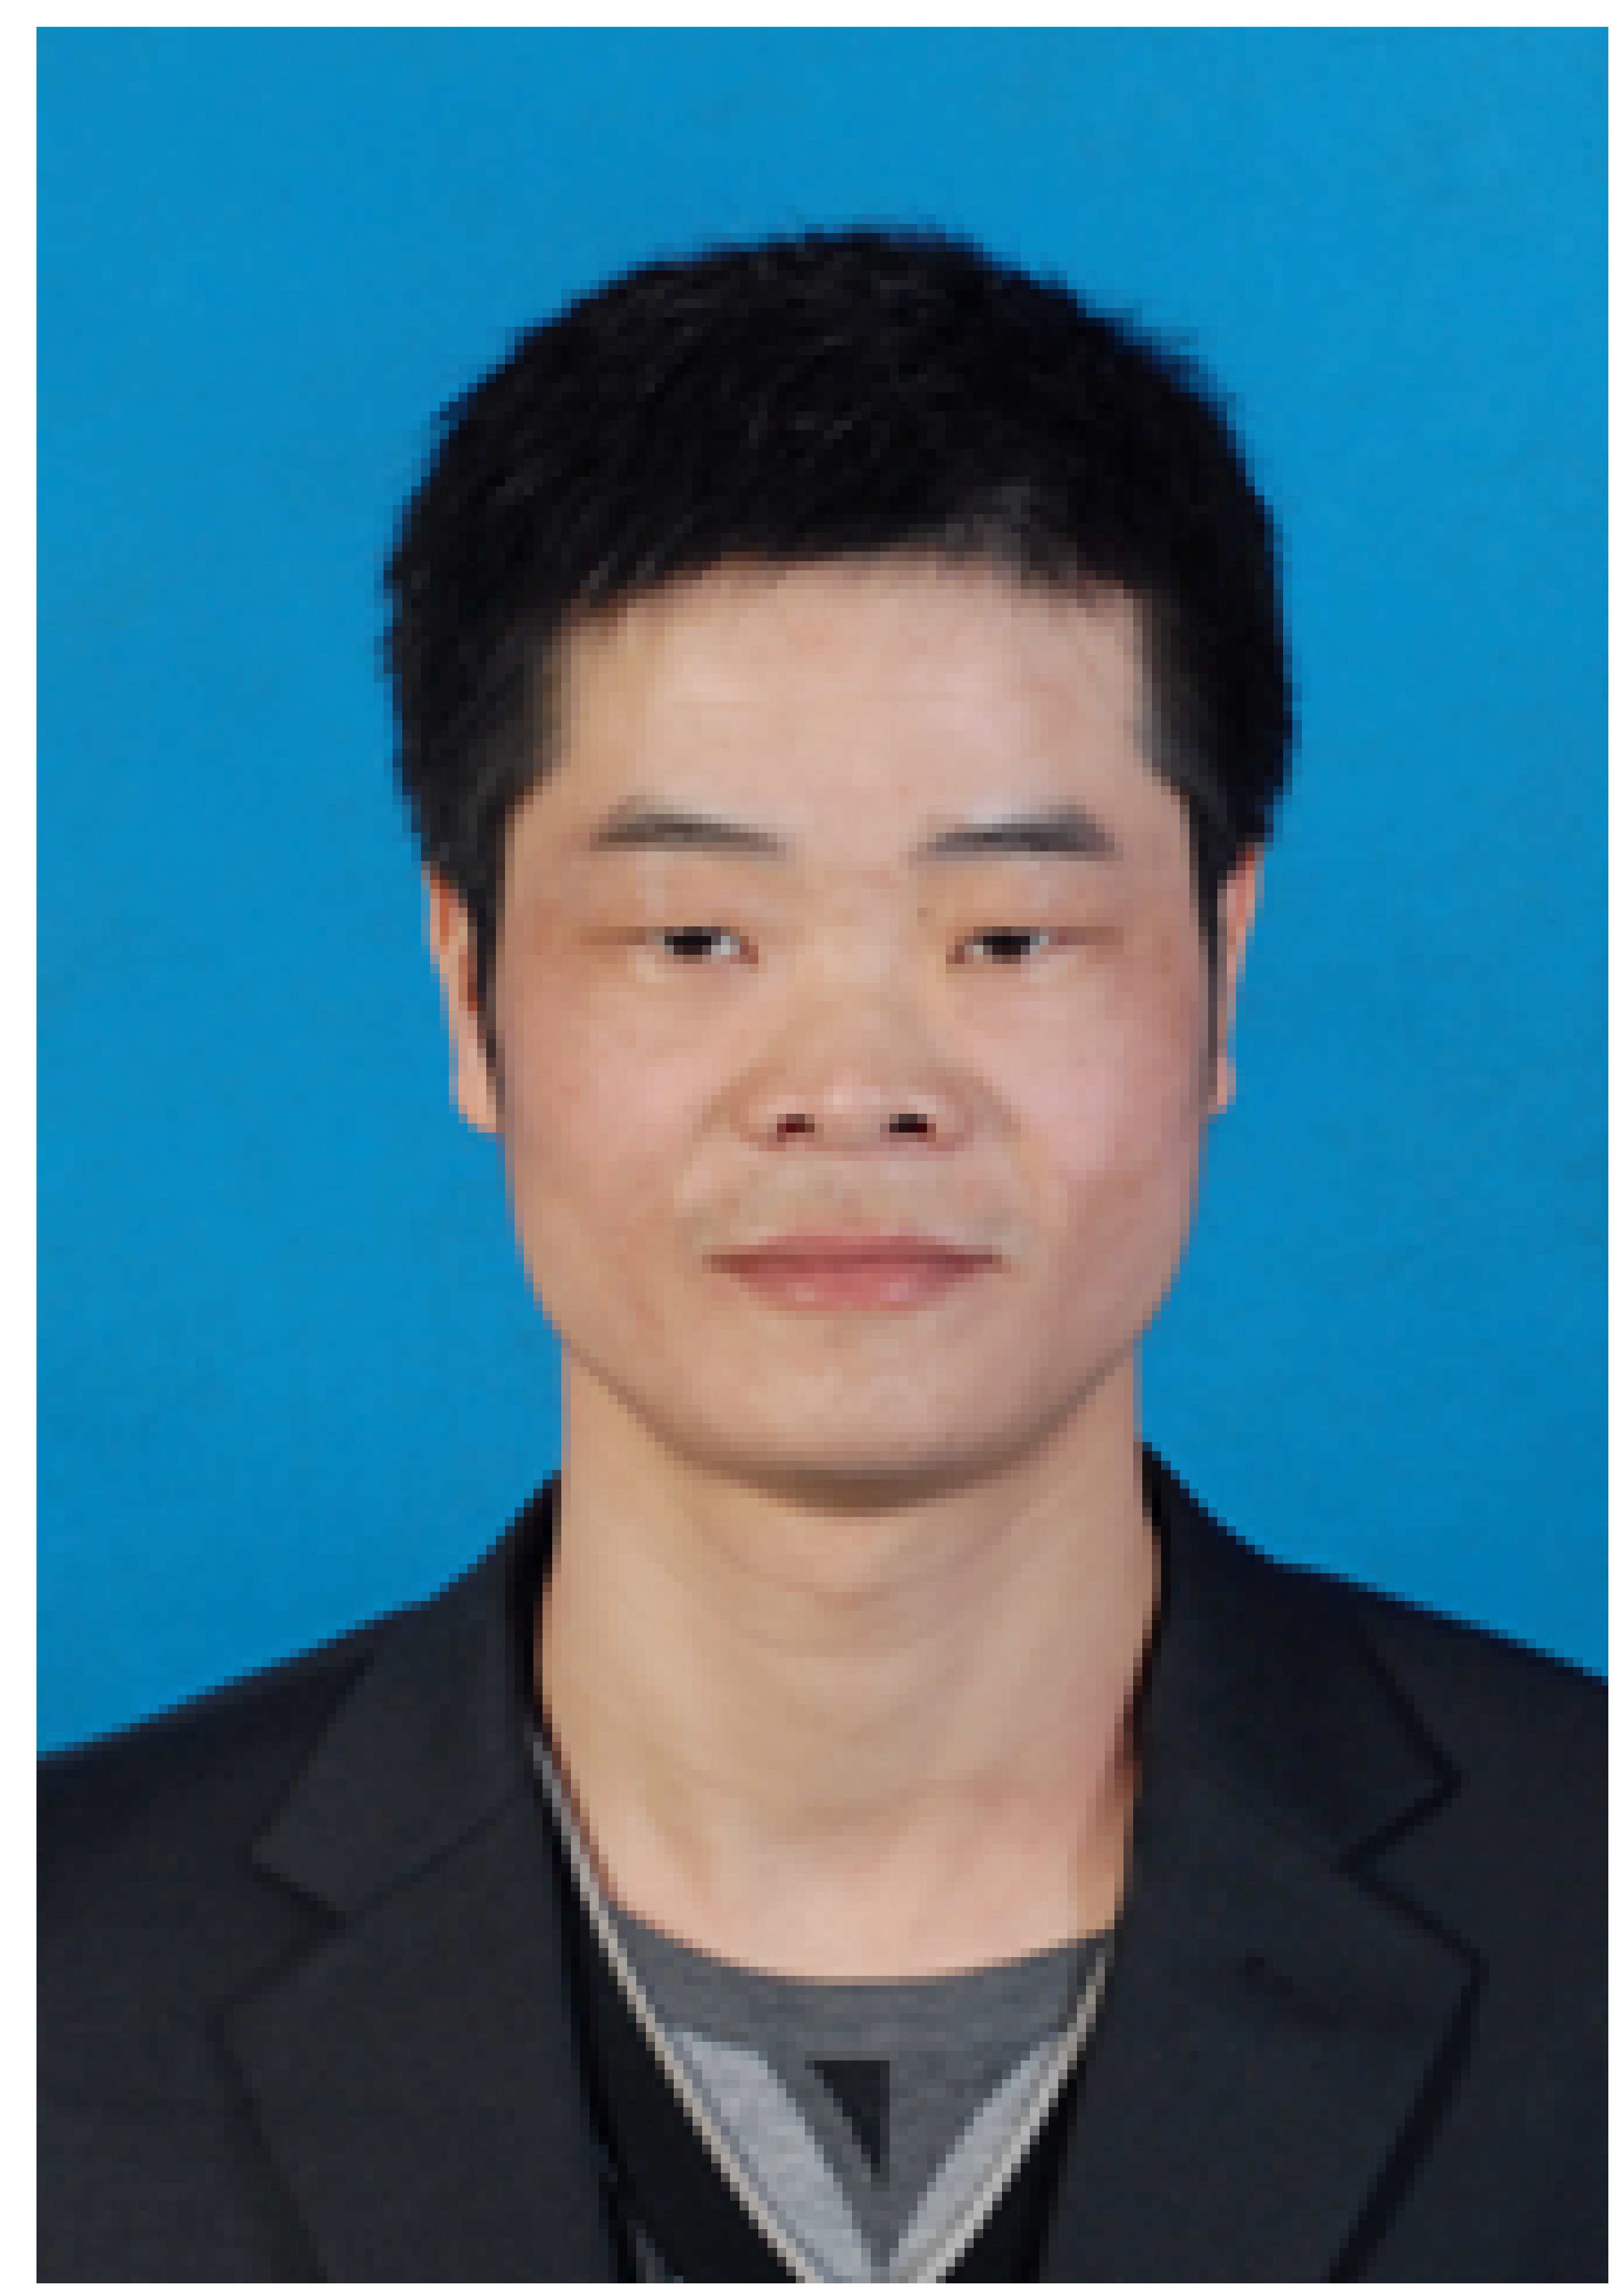
\includegraphics[width=1in,height=1.25in,clip,keepaspectratio]{author2-yangzb.eps}}]
{Zhibang Yang}
received the PhD degree in computer science from Hunan University, Changsha, China, in 2012. He is currently an associate professor at Changsha University. His research interests include cybersecurity, industrial control systems, and edge-cloud computing.
\end{IEEEbiography}
\vspace{-2mm}
\begin{IEEEbiography}[{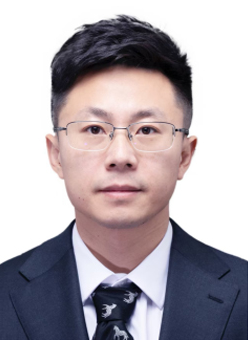
\includegraphics[width=1in,height=1.25in,clip,keepaspectratio]{yumeng.png}}]{Yumeng~Liu} 
received the PhD degree from the Institute of Software, Chinese Academy of Sciences, Beijing, China, in 2023. He is a senior engineer at the Institute of Software, Chinese Academy of Sciences. His research interests include data mining and database technology.
\end{IEEEbiography}
\vspace{-2mm}
\begin{IEEEbiography}[{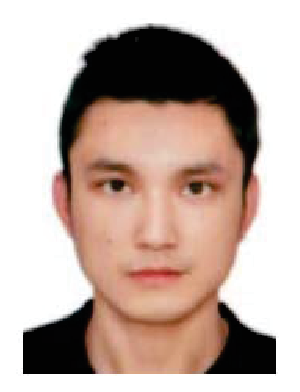
\includegraphics[width=1in,height=1.25in,clip,keepaspectratio]{author3-yusiyang.eps}}]{Siyang Yu} 
	received the PhD degree in computer science and technology from Hunan University, China, in 2017. He is currently a faculty member at Hunan University of Finance and Economics. His research interests include the industrial Internet of Things, anomaly analysis, and intrusion detection.
\end{IEEEbiography}
\vspace{-2mm}
\begin{IEEEbiography}[{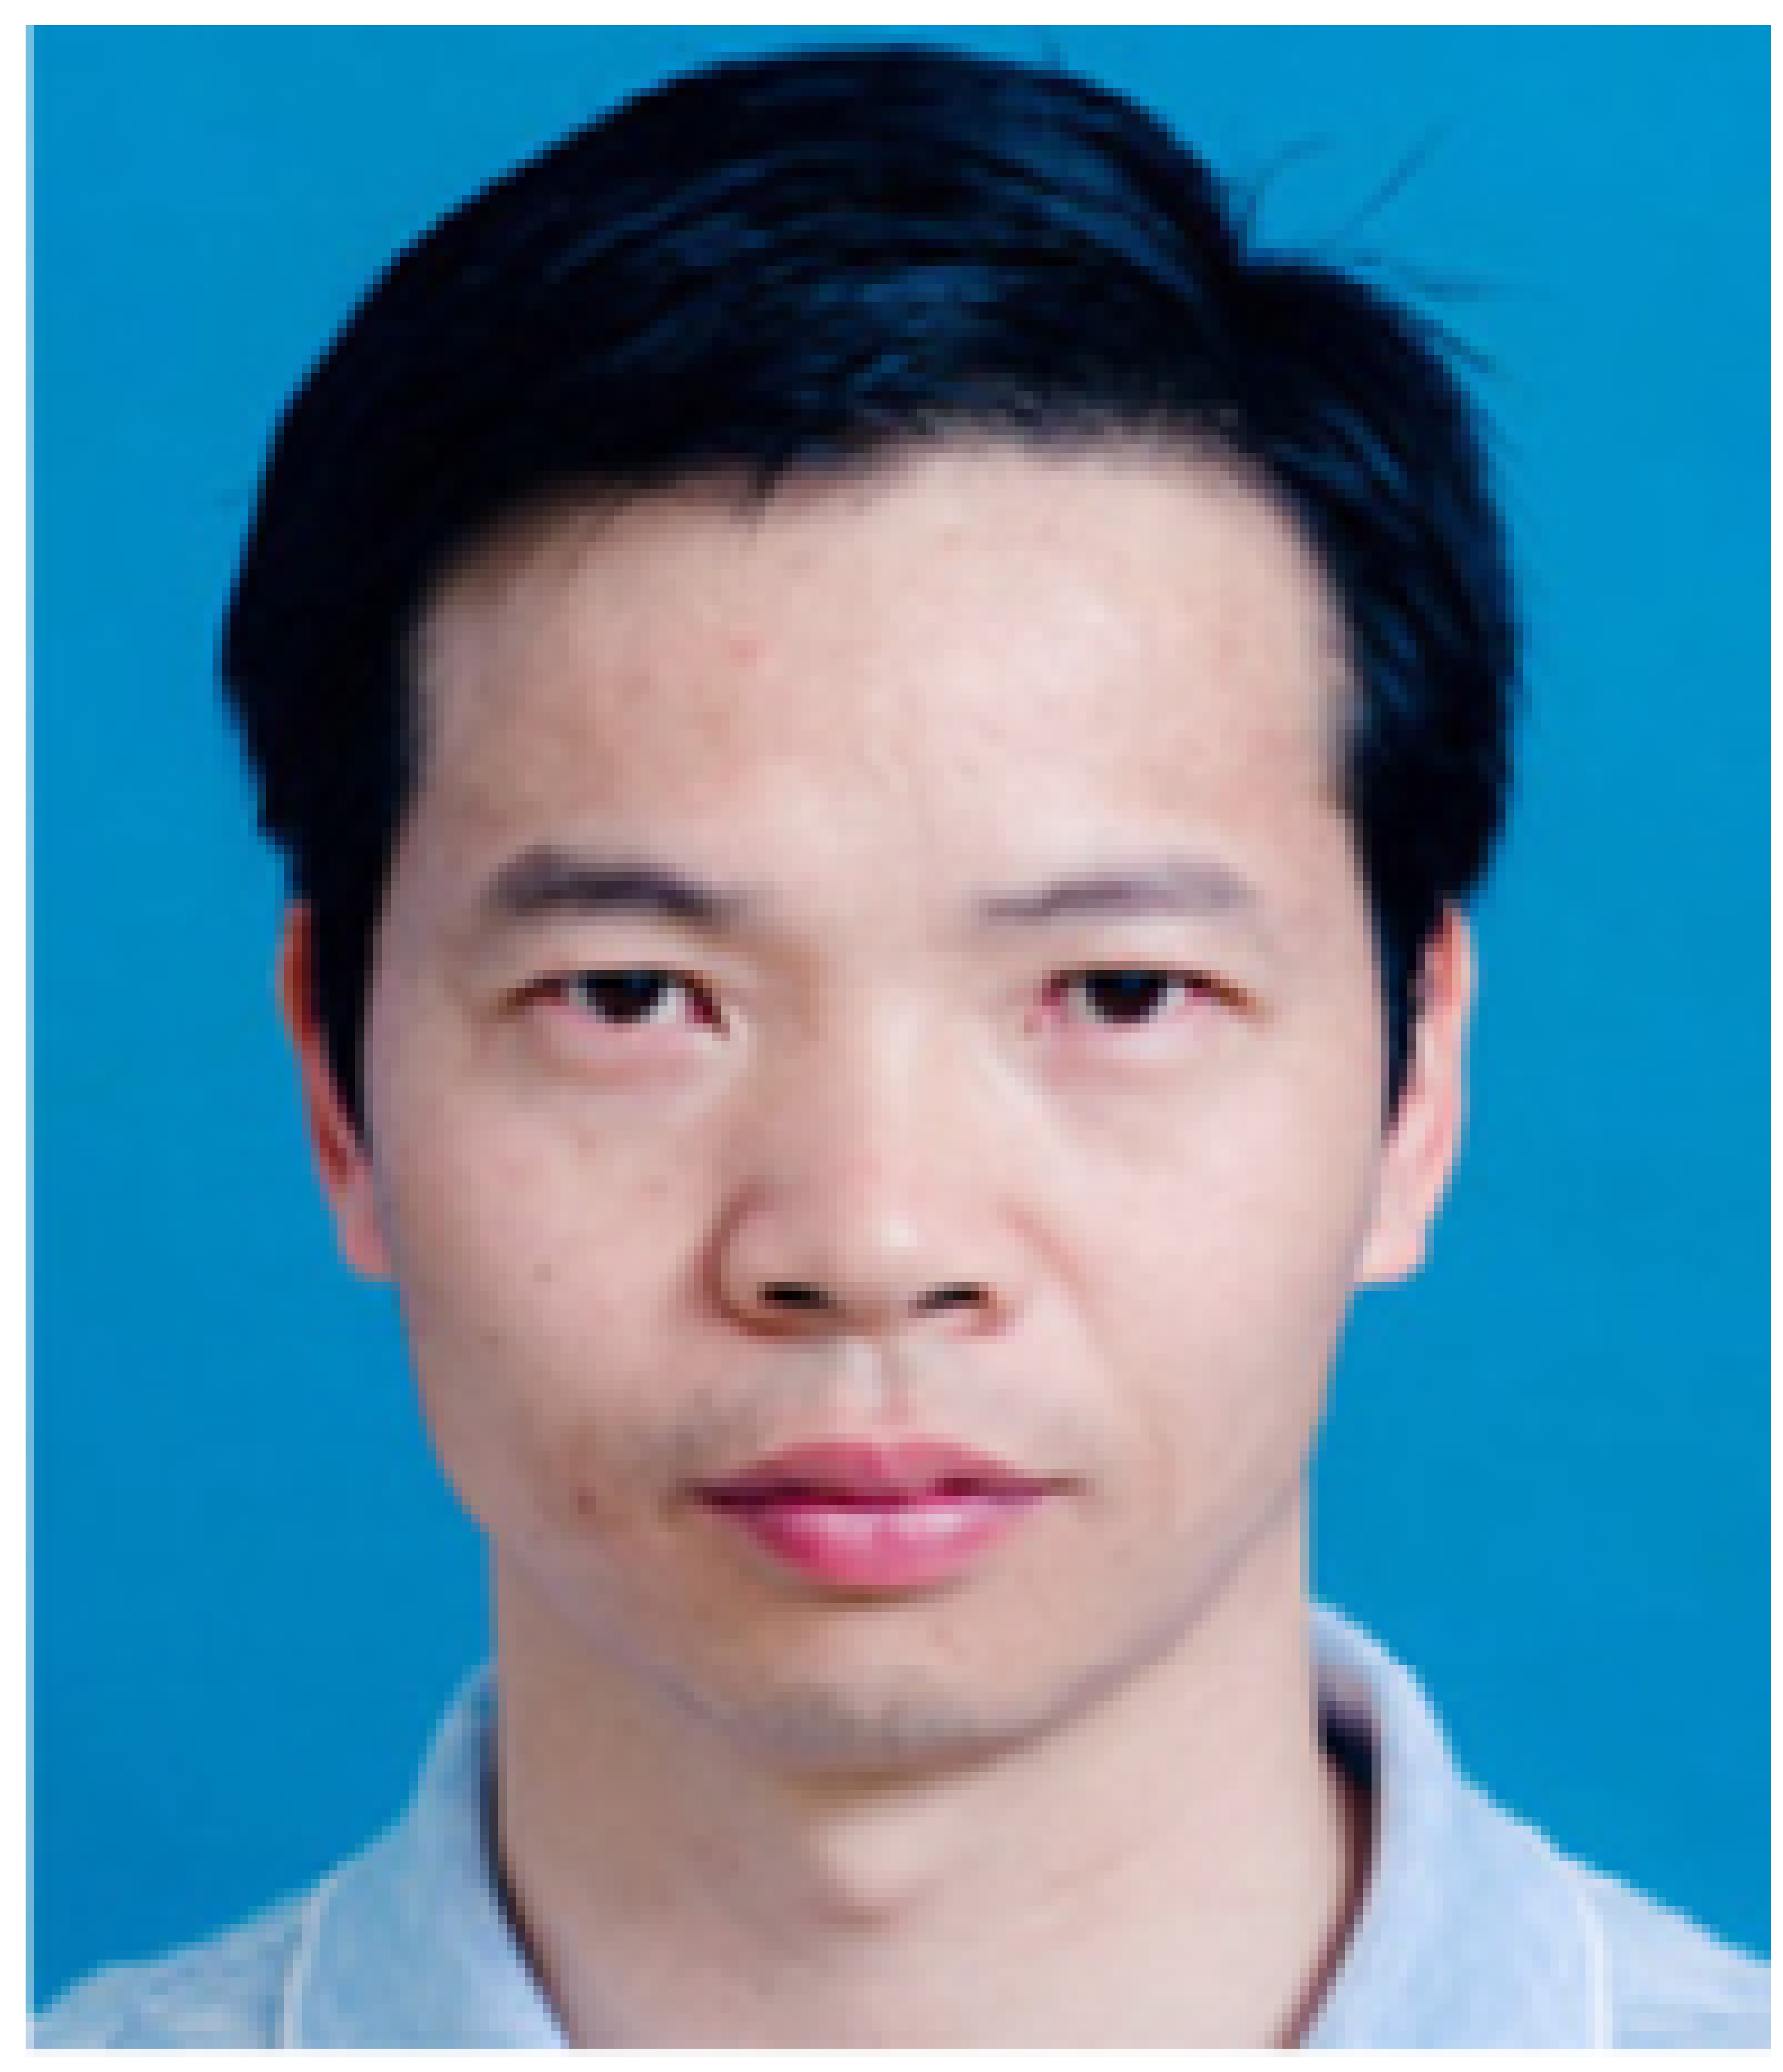
\includegraphics[width=1in,height=1.25in,clip,keepaspectratio]{author4-liKenli.eps}}]{Kenli Li}
	received the PhD degree in computer
	science from Huazhong University of Science
	and Technology, China, in 2003. He is currently a Cheung Kong professor of computer science and technology with Hunan University and the dean of the College of Computer Science and Electronic Engineering, Hunan University. His research interests include parallel and distributed processing, high-performance computing, and big data management. He has published more than 250 research papers
	in international conferences and journals such as TC, TPDS, TCC, ICPP, ICDCS, etc.
	He serves on the editorial board of the IEEE-TC. He is an outstanding member of the CCF and a senior member of the IEEE.
\end{IEEEbiography}





\end{document}
